%!TEX root = ../../thesis.tex

\subsection{The anatomy of an event}

\ac{MC} event generators provide fully-exclusive hadron-level simulation of \pp collision 
events at the \acs{LHC} \cite{MCnet:general}. \Figure~\ref{fig:mcevent} shows how event 
generation is factorised into several components, each describing a certain regime of 
momentum transfer.

\begin{figure}[b]
	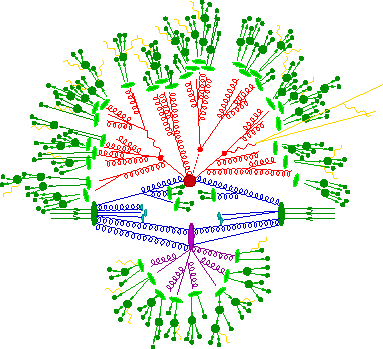
\includegraphics[width=\mediumfigwidth]{tex/tools/event}
	\caption{Schematic diagram of a simulated \ttH event, showing how factorisation allows 
	the physics at different scales of momentum transfer $Q$ to be treated independently 
	\cite{MCnet:MatchingLectures}.
	At high-$Q$ is the hard scatter (red circle). As the scale evolves down, partons are 
	radiated in the initial state (blue) and final state (red). At low-$Q$, incoming 
	partons are confined to the beam protons, while outgoing partons hadronise (light 
	green blobs). The underlying event contains multiple partonic interactions (purple 
	blob) and beam remnants (light blue blobs). Photons (yellow) are also radiated.}
	\label{fig:mcevent}
\end{figure}

\begin{description}
\item[Hard scatter] \hfill \\
	The high scale process is selected by the user (\eg Higgs boson production via 
	gluon-gluon fusion). The relevant parton-level \acp{ME} are calculated using fixed 
	order perturbative QCD, either by the event generator itself or an external program. 
	These \acp{ME} are usually \ac{LO}, though possible improvements are discussed in 
	\Section~\ref{sec:mc:merging} and \Section~\ref{sec:mc:matching}.
\item[Parton Distribution Functions (PDFs)] \hfill \\
	Incoming parton momenta are sampled from a proton \ac{PDF}, usually probed at the 
	scale of the hard scatter $\mu_F = Q$. The LHAPDF interface \cite{LHAPDF} provides 
	access to the \acp{PDF} of several fitting collaborations, such as CTEQ \cite{CTEQ} 
	and MSTW \cite{MSTW}.
\item[\ac{FSR}] \hfill \\
	Soft and collinear radiation from outgoing partons is simulated by a universal parton 
	shower, evolving the scale from the hard scatter to the hadronisation scale of 
	\about\unit{1}{\GeV}. The successive emissions are ordered to avoid double-counting -- 
	common order parameters are virtuality, transverse momentum and opening angle.

	For the correct treatment of soft emissions, it is vital to preserve coherence. This 
	is inherent in an angular ordered shower, but must be manually implemented otherwise. 
	Alternatively, a \textit{dipole shower} considers emissions from colour-connected 
	pairs of partons, and is also inherently coherent.
\item[\ac{ISR}] \hfill \\
	universal, soft collinear limit, perturbative, summed to all orders, backwards evolution
\item[Hadronisation] \hfill \\
	universal, non-perturbative, cluster and Lund string models
\item[Hadronic decay] \hfill \\
	dumdeedoo
\item[\ac{MPI}] \hfill \\
	process dependent, non-perturbative, various models
\item[\acs{QED} radiation] \hfill \\
	dumdeedoo
\end{description}

\subsection{Summary of event generators}
\begin{description}
\item[Herwig] \hfill \\
	\fherwig or \herwigpp \cpp
\item[Pythia] \hfill \\
	\pythia{6} or \pythia{8}
\item[\sherpa] \hfill \\
	\sherpa
\end{description}

\subsection{ME-PS merging}
\label{sec:mc:merging}

\begin{description}
\item[CKKW] \hfill \\
	dumdeedoo
\item[MLM] \hfill \\
	dumdeedoo
\end{description}

\subsection{NLO-PS matching}
\label{sec:mc:matching}

\begin{description}
\item[\mcatnlo] \hfill \\
	dumdeedoo
\item[\powheg] \hfill \\
	dumdeedoo
\end{description}

\subsection{Additional considerations}
\begin{description}
\item[Pile-up] \hfill \\
	in-time/out-of-time pile-up
\item[Detector simulation] \hfill \\
	GEANT4
\end{description}